\begin{center}
\textsc{\Large Laboratorio 5}~\\
{\large Vídeo Juegos, Programación, Físicas}~\\
\emph{Detección de Colisiones}
\end{center}


\section{Pre-Laboratorio}
\begin{itemize}
\item Investigar los siguientes conceptos:
\begin{enumerate}
  \item Arquitectura Sistemas-Componente-Entidad (Entity Component Systems o ECS), ver como esta puede ser utilizada para el desarrollo de vídeo juegos en general.
  \item Octrees y quadtrees, arboles BSP y sus usos.
\end{enumerate}
\item Explique al menos dos casos para los que se podría utilizar detección de colisiones en un vídeo juegos.
\item Investigue para su herramienta de trabajo escogida como incorporar colisiones, si este ya posee detección de colisiones o debe ser incorporado a través de bibliotecas.
\end{itemize}

\section{Definición}
Consiste en el problema computacional de detectar la intersection entre dos o mas objetos. Ademas de detectar si dos objetos interceptan un sistema de colisión de objetos puede reportar tiempo y punto de impacto \cite{ericson_collision}.

En una simulación física de colisiones se busca imitar la colisión entre uno o mas objetos de la forma mas precisa posible siguiendo las características físicas de los objetos en cuestión y las distintas propiedades de los materiales que los componen utilizando cuerpos rígidos (rigid-body physics) o cuerpos blandos (\emph{soft-body physics}) \cite[p.~340]{jenkinscreatinggames}.

Mientras en un vídeo juego se busca simular colisiones de una forma aceptable, en tiempo real y robusta.

\section{Intersecciones Objeto / Objeto}
Real Time Rendering: Intersections Object / Object \url{http://www.realtimerendering.com/intersections.html}. Este sitio presenta referencias a soluciones de intersecciones objeto / objeto, la mayoria de estas soluciones se encuentran en la serie \emph{Graphics Gems}. Muchos frameworks y bibliotecas para el desarrollo de vídeo juegos (o software general) ya tienen estas soluciones implementadas e incluso optimizadas \cite{rtr_intersections}.
\section{Tecnicas y Optimizaciones Comunes}
\subsection{Partición Espacial (Spatial Partitioning)}
\setlength\intextsep{0pt}
\begin{wrapfigure}[12]{l}{0.3\linewidth}
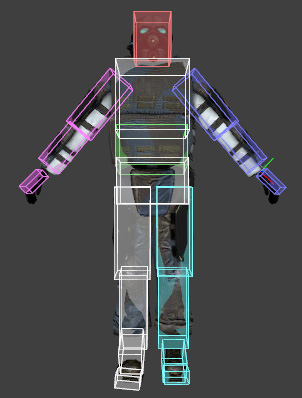
\includegraphics[width=\linewidth]{media/Hitbox.jpg}
\caption{Hitboxes de un \emph{Combine} de \emph{Half Life 2} \cite{valve_hit} \cite{halflife2}.}
\label{fig:hitboxes}
\end{wrapfigure}
Existen una variedad de algoritmos utilizados para dividir un espacio virtual entre los mas comunes están los octrees, quadtrees y arboles BSP (binary space partitioning). Esta partición espacial se realiza para evitar determinar intersecciones entre objetos que no pertenecen a una misma área determinada por el algoritmo de partición espacial, de esta forma se disminuye el numero de comparaciones aumentando el desempeño o \emph{performance} \cite{sp_partition}.
\subsection{Bounding Boxes o Bounding Volumes}
Usualmente rectángulos en 2D o cubos en 3D pero también es posible usar otras figuras como esferas, círculos, elipses, paralelogramos, envolventes convexas entre otras. Son usadas como un inicial test de colisión de tal forma que solo se determina la intersección con objetos dentro del bounding volume \cite{douglas_bbox}.
\subsection{Hit Boxes}
Al igual que un Bounding Box estos suelen ser cubos o rectángulos pero también pueden ser otras figuras, el uso de elipses o elipsoides es común. Para objetos animados es usual que los hit boxes estén enlazados a las partes que se mueven de tal forma que los hit boxes también se muevan y roten en correlación con el personaje u objeto al que pertenecen. Los hit boxes son utilizados para detectar colisiones unidireccionales como un objeto en intersección con un bala u otro proyectil. Son poco precisos para colisiones con \emph{feedback} como chocar contra una pared ya que la posición y orientación de los hit boxes cambia constantemente, este tipo de colisiones son mejor manejadas por bounding boxes alineadas a un eje \cite{valve_hit}. 

\section{Actividad}
En esta actividad debe incorporar distintas acciones y eventos que hagan uso de detección de colisiones.
\begin{itemize}
\item Debe incorporar detección de colisiones para las siguientes condiciones.
\begin{enumerate}
  \item Jugador principal contra actores con movimiento.
  \item Jugador principal contra objetos inamovibles.
  \item Jugador principal contra objetos en movimiento.
  \item Actor con movimiento contra objetos inamovibles.
  \item Actor con movimiento contra objetos en movimiento.
  \item Actor con movimiento contra actor con movimiento.
\end{enumerate}
 \item Debe crear un sistema de historial de eventos donde cada colisión e información de la misma es guardada. Considere como datos necesarios, tiempo de colisión e información de ambos objetos en colisión. Debe agregar mas datos del evento de colisión que vea de utilidad para su mecánica y diseño de juego.
\end{itemize}